\chapter{Model Force-Calcium}
\label{chap:force_calcium}
 
\section{Introduction}

The relation betweem membrane depolarization ($V_m$) to $\Ca$ transient to force
generation is important for normal function of the heart. The molecular origin
of the force produced between myosin and actin is one of the outstanding puzzle
in biology. Our current understanding of the mechanism of contraction is based
on three fundamental discoveries \citep{szent-gyorgyi2004}:
\begin{enumerate}
  \item Contraction is the result of the interaction of two proteins (actin and
  myosin) with ATP. Thus, contraction can be reproduced {\it in vitro} using
  purified proteins.

  \item The shortening of the cell and the constant length of both
  filaments (thick and thin filaments) during contraction is explained by the
  {\it sliding filament theory}. Each filament contains hundreds of
  molecules and the contraction is caused by sliding, without any change in
  filament lengths \citep{cooke2004}. It explains the constancy of A-band and
  the changes of I-band and H-zone.

  \item The search for molecular structure changes during force production can
  be done thanks to the available of atomic structures arising from
  crystallization of actin and myosin \citep{rayment1993}.
\end{enumerate}

The formation of swinging cross-bridge, i.e. the head of the thick filament
(whose monomer is myosin) bind to the thin filament (whose monomer is actin)
driven by ATP hydrolysis and calcium binding which has been clearly visualized
using electron microscopy of ultra-thin sections by Huxley
\citep{huxley1957,huxley1974}.
The widely accepted hypothesis of muscle contraction is that force is developed
when the cross-bridge is form \citep{huxley1954}. This conformational change in
the attached cross-bridge produces a pulling force on the thin filament toward
the center of a sarcomere \citep{geeves2005}. This interaction happens when a
free $\Ca$ binds to troponin C (TpnC), exposing the actin monomer of the thin
filament to the cross-bridge \citep{ford1991}, and an ATP molecule is hydrolized
to bend the myosin head. We'll discuss in details in the next subsections.

\subsection{Myosin \& Actin}

The term myosin given to the protein discovered by Kuhne (1864).
In 1939, Engelhardt and Luybimova showed that myosin has ATPase activity. In
1940s, it was then shown that the proteins they have been studied were actually
2 myosins: myosin A (low viscosity) and myosin B (high viscosity). The viscosity
of myosin B is reduced by adding ATP.
The difference was accounted for the involvement of a third protein, called {\bf
actin} which is responsible for the high viscosity. Myosin A retains the name
{\bf myosin}, and myosin B combined with actin was called {\bf actomyosin}
(since 1942) (for review \citep{szent-gyorgyi2004}).
\textcolor{red}{Multiple dimers of myosin forms the thick filament, by
overlapping in a helical fashion around the long axis of the filament.
In many books, myosin filament is used to refer to thick filament}.
Each thick filament consists of about 200-400 myosin molecules
\citep{hanson1963}
\url{http://library.thinkquest.org/C003758/Function/How Cardiac Muscle
Contracts.htm}.

Nowadays, there are so many types of myosin (at least 18 types): myosin I,
myosin II, etc. with a huge diversity in structure and mechanochemical
properties \cite{hodge2000, berg2001}
(web reference: \url{http://www.mrc-lmb.cam.ac.uk/myosin/myosin.html}). Myosin
II (aka the conventional myosin) is the one involving in muscle contraction
\citep{cooke1997}.
Myosin II has 2 heavy chains, and two sets of light chains (ELC and RLC)
wrapping around the myosin heads, Fig.\ref{fig:myosin_II} (A). Phosphorylation
can occur on the light chain and the C-terminus of the heavy chain. Another
separatin of myosin into 2 components: LMM and HMM, Fig.\ref{fig:myosin_II}(B).
LMM is fully coiled $\alpha$-helix (with the estimated length $\sim 900 \AA$
\citep{huxley1963}) and is resonsible for filament formation, where HMM contains
the sites responsible for ATPase activity and sites for interacting with actin.
At low ionic strengths, LMM form paracrystals, while HMM remained fully soluble.
The 64-residues long region between LMM and HMM  was suggested that it lacks the
coiled coil structure. HMM is divided into 2 subfragments: S1 and S2.

\begin{figure}[hbt]
  \centerline{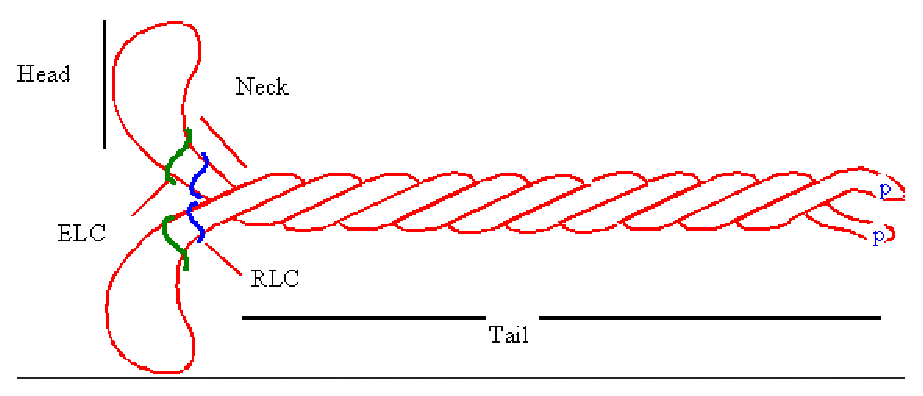
\includegraphics[height=3cm,
    angle=0]{./images/myosin_II.eps}}
      \centerline{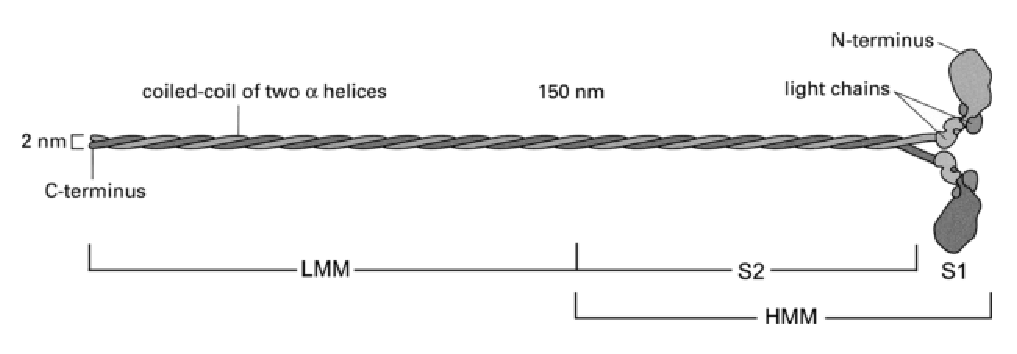
\includegraphics[height=3cm,
    angle=0]{./images/myosin_molecule.eps}}
\caption{A myosin molecule with 2 heavy-chains and 2 sets of light-chains: ELC =
essential light chain, RLC = regulatory light chain. The slow component is
light meromyosin (LMM) and faster component is heavy meromyosin
(HMM)\citep{szent-gyorgyi2004}}
\label{fig:myosin_II}
\end{figure}

In cardiac cell, the myosin head is the globular motor domain, aka cardiac
$\beta$-myosin heavy chain\footnote{\url{http://ghr.nlm.nih.gov/gene/MYH7}}. The
protein is encoded by MYH7 gene. The tail domains of each heavy chain interact
to form a rod-like $\alpha$-helical coiled coil. The light chains are similar to
Calmodulin in structure; it has regulatory role, and stiffen the neck regions.
The binding site for each light chain is an IQ motif (isoleucine, glutamine):
IQxxxRGxxxR. The neck region in muscle myosin consists of a central
$\alpha$-helix with a variable number of IQ motifs (zero to six).


Actin was discovered by Straub in 1942. In 1943, Straub showed that actin has 2
forms: G-actin (globular actin) and F-actin (the polymerized (fibrous) form of
G-actin in the presence of ions). The protein actin is one of the most highly
conserved proteins during evolution (80.2\% gene sequence conservation, and 90\%
primary structure conservation of the protein product). Action is about
1.95$\mum$ \citep{page1968}. \textcolor{red}{Actin molecules, combining with
Tropomyosin and Troponin, constitute the thin filament. In many books, the thin
filament is often called actin filament}. The number of actin monomers in the
thin filament is about the same number as myosin molecules in thick filament.
Sect.\ref{sec:troponin} will discussed Troponin proteins.
A computational study on actin typically assume either one of the two approaches
\begin{itemize}
  \item 2-state: blocked and open (when calcium binds to TnC)
  \item 3-state: blocked, closed (when calcium binds to TnC, but not
  physically move the molecule) and open (calcium bound and the Troponin is
  moved to reveal the active sites).
\end{itemize}


\subsection{Troponin}

Sect.\ref{sec:troponin}
%\label{sec:troponin}


\subsection{Sarcomere}
\label{sec:sarcomere}
\label{sec:contractile-unit}

\begin{figure}[hbt]
  \centerline{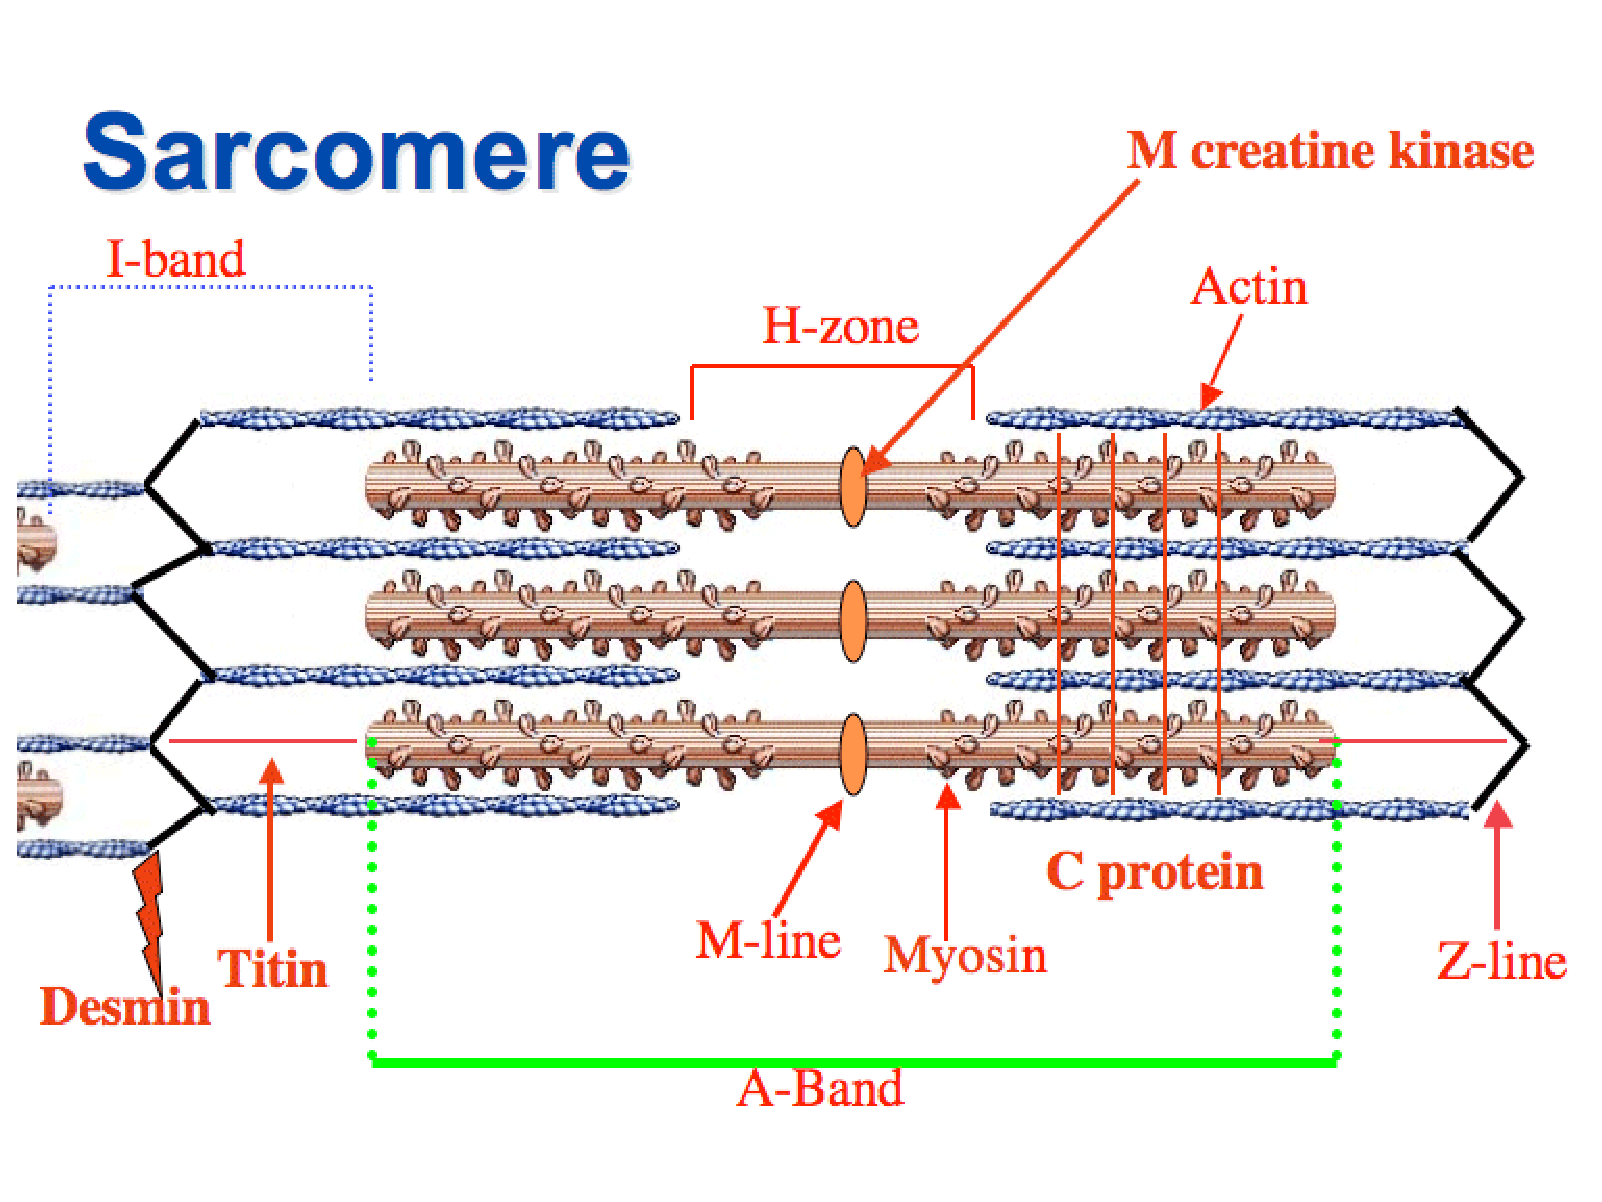
\includegraphics[height=6cm,
    angle=0]{./images/sarcomere3.eps}}
\caption{A sarcomere extends from one Z-line to the next Z-line. The distance
between 2 Z-lines is about 2-3$\mum$}
\label{fig:sarcomere3}
\end{figure}

Each cross-striated muscle is organized in sarcomeres, repeating units in about
2-3$\mum$ long. A sarcomere is the basic of {\bf contratile unit}, limited by 2
prominent Z-disc (or Z-line), Fig.\ref{fig:sarcomere3} and
Fig.\ref{fig:sarcomere}.
Sarcomere, is considered as the building block of muscles, plays a critical
role in muscle contraction.


In between is the number of components, e.g. thick filaments and thin filaments.
The monomer of thick filament is myosin and the main constitutients of thin
filament is actin, Fig.\ref{fig:thick_thin_filament}. Thick filaments
(1.6$\mum$) spanning across a region known as A-band and thin filament (1$\mum$)
streatching from Z-line to one end of H-zone. The region with Z-line as the
center, and contains no thick filament is called I-band. The central bare zone
in which there are no cross-bridges is known as H-zone.
The central area of the A-band is known as M-line, which contains {\it M
creatinine kinase} which involves in catalytic activity
\begin{equation}
\ce{ATP + creatine = ADP + phosphocreatine}
\end{equation}

\begin{figure}[hbt]
  \centerline{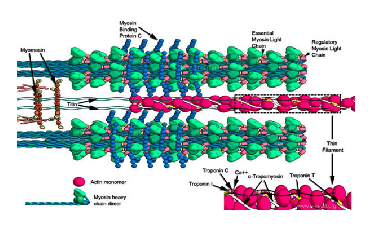
\includegraphics[height=6cm,
    angle=0]{./images/thick_thin_filament.eps}}
\caption{Myosin is the monomer that forms thick filament
\footnote{\url{http://www.e-heart.org/pages/01_cardiac_structure/01_Cardiac_Structure_Molecular_Anatomy_002.htm}}}
\label{fig:thick_thin_filament}
\end{figure}


Another protein, {\it myomesin}, can serve as a molecular spring to protec the
sarcomere and keep it stabilize during intense or sustained stretching
\citep{schoenauer2005}. The rod portion (light meromyosin) of thick filament
insert in the lattice formed by myomesin and other molecules in the M-line.
There is an important protein, {\it titin} (the largest known protein), which
connect the Z-line to the M-line and anchor the thick filament. This aims to
transmit at the Z-line when thin filament sliding over thick filament; and also
limit the range of motion of the sarcomere in tension, contributing to the
passive stiffnes of the muscle.

Each myosin has a 'hinge' region that allows the molecule to bend. At the end of
this hinge region is the myosin head which interacts with actin in a reaction
cycle forming cross-bridge. There are 4 stages of cross-bridge cycle,
Fig.\ref{fig:myosin_cross-bridge}. The contraction is driven by cross-bridge
activity.  At resting, myosin stays at a low-energy conformation, in which ATP
bind to the cleft at the 'back' of the head of myosin (7-stranded $\beta$-sheet)
so that myosin cannot interact with actin. When ATP is hydrolyzed (into ADP+Pi),
the head now can swing back about 5nm to the 'cocked' position.

Pi then leaves the myosin, leading to the binding of myosin to actin. At almost
the same time, calcium bind to TnC, and then tropomyosin (Tm, another protein in
the thin filament) moves out of the way of the active actin site, allowing
myosin head to bind to thin filament. Finally, ADP is released to generate the
'power stroke', causing the cell to contract
\footnote{\url{http://www.bms.ed.ac.uk/research/others/smaciver/Myosin II.htm}},
before ATP rebinds to release the cross-bridge forming. During the contraction,
actin filament move towards the center from both halves of the sarcomeres.

\begin{figure}[hbt]
  \centerline{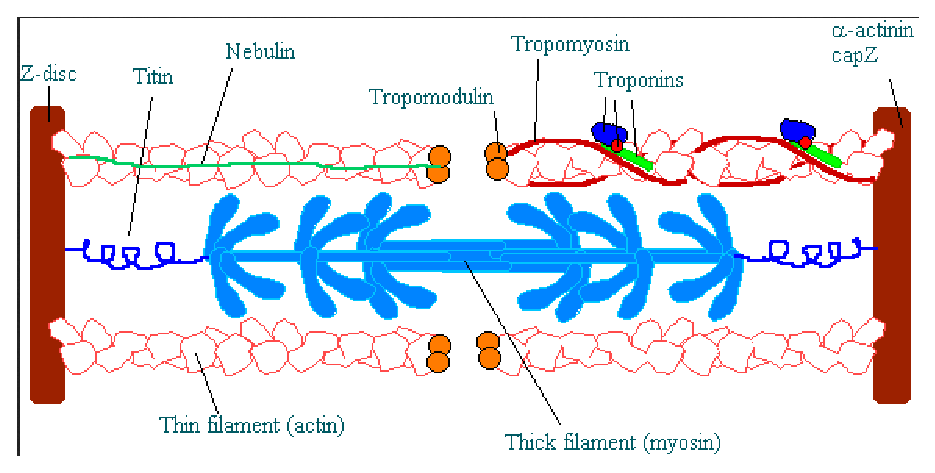
\includegraphics[height=3cm,
    angle=0]{./images/sarcomere.eps}}
\caption{Thick filament (blue), thin filament (red). Titin is an enormous
spring-like molecule. The distance between 2 Z-disc at relaxation is 2.5mm}
\label{fig:sarcomere}
\end{figure}

\begin{figure}[hbt]
  \centerline{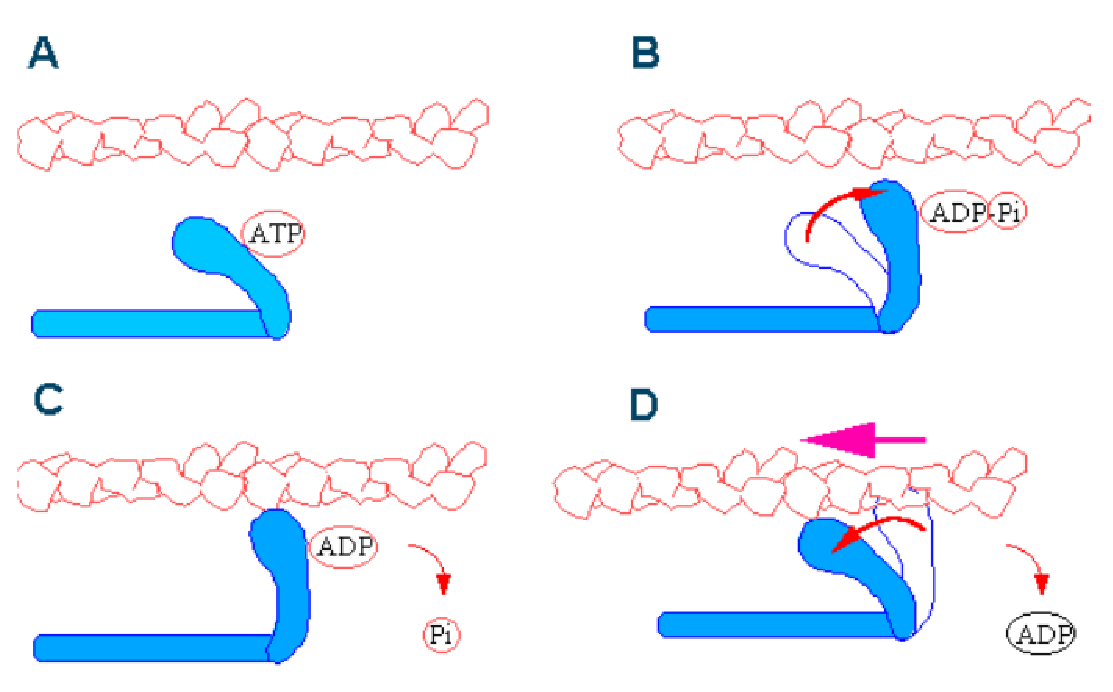
\includegraphics[height=3cm,
    angle=0]{./images/myosin_cross-bridge.eps}}
\caption{4 stages in Myosin Cross-bridge Cycle}
\label{fig:myosin_cross-bridge}
\end{figure}




\subsection{Contraction converts chemical energy to work}


It's the change in membrane potential that drive contraction of the fibre
\citep{kuffler1946}. The membrane potential propagate along the surface membrane, and also inwards along
the membranes of the tubules, which constitute the 'T' (tranverse) system. In
amphibians, there's one transverse network per sarcomere (at Z-line); while in
mammals there are two transverse network per sarcomere (each one near each
boundary between A-band and I-band) \citep{page1969}.

Muscle is a machine that convert chemical energy into work; at which ATP is the
link between metabolism and contraction where the energy factories are mitochondria.
ATP is synthesized from ADP and inorganic phosphate via glycolytic and oxidative
metabolism in mitochondria (Sect.\ref{sec:ATP-synthesis}).

Glycolysis (a sequence of 10 reactions) is the process converting glucose into
pyruvate (\ce{CH3COCOO-} a key intersection in several metabolism pathways) and
proton (\ce{H+}). When oxygen is present, pyruvate supplies energy (i.e. ATP and
NADH) through Krebs cycle (citric acid cycle); and produce lactic acid
otherwise.

Glycolysis is the
breakdown of glycogen to lactic acid. Early evidences suggested that lactic acid
is good for muscle contraction, and a factor causing fatigue in muscle
\citep{needham1971}.
Later studies suggested that lactic acid can help muscle contract more
efficiently \citep{pedersen2004}.
\begin{equation}
\ce{n(C6H12O6) -> 2n(C3H6O3)}
\end{equation}
Muscle cells convert gluose and glycogen into lactic acid which is taken up and
used as fuel by mitochondria. [Atheletes training on improving endurance helps
increasing the mass of muscle mitochondria, letting the burn more lactic acid
and allowing muscle to work harder and longer].

Recent evidences giving some evidences why muscle become tired, i.e. tiny
channels on the membrane start leaking calcium, and that weaken contractions.
Also, leaked calcium stimulates an enzyme that eats into muscle fibers,
contributing to muscle exhaustion.

In 1929, German biochemist Karl Lohmann discovered adenosine triphosphate (ATP)
as the key source of
energy\footnote{\url{http://www.nndb.com/people/075/000249325/}}. In 1935,
Lohmann found that ATP and creatinine phosphate (Phosphorylcreatine or PCr) are
held in equilibrium by creatine kinase which we call it {\it Lohmann reaction}
\begin{equation}
\ce{ADP + PCr <=>[\text{creatine kinase}] ATP + creatine}
\end{equation}
with $K_\eq \approx $ 20 to 100.  When ATP is produced (oxidation of food), the
equilibrium shifts to the left, forming PCr. When ATP is needed or ADP is
available in a large amount, the equilibrium shift to the right. This enables a
large quantities of ATP to be available on a short time scale.

Both the first and second law in thermodynamics can be applied to muscle, i.e.
427.263 kg.m = 1.000 kilocalories = 4.184
kilojoules\footnote{\url{http://www.uic.edu/classes/phyb/phyb516/energeticsu3.htm}}.

\begin{framed}
However, ATP
concentration in muscle is quite low (5-8$\muM$/g muscle), only enough for a few
contraction. The used ATP can be resynthesized from PCr. Yet the low
concentration of PCr (20-25$\muM$/g) is only enough for some additional
contraction. Glycogen offers a rapid way of synthesizing ATP, but still limited
energy store (endogenous glycogen concentration is about 75$\muM$/g muscle).
The most efficient process for ATP production is oxidative
phosphorylation \citep{paul1993}.
\end{framed}

\subsection{Model contraction}

Early models tried to develop a relationship between force strength vs.
sarcomere length. The first model of a motor protein was proposed by Sir Andrew
Huxley (1957), Fig.\ref{fig:motor_protein_Huxley}, before the myosin
cross-bridge had been visualized. In this model, the relaxation of the spring
provides the enthalpy to perform mechanical work of the power stroke. At the end
of the power stroke, myosin is bound tightly to the actin. This bond can be
borken by the binding of ATP to the myosin. Here, the random thermal fluctuation
is mapped to unidirectional mechanical work.

\begin{figure}[hbt]
  \centerline{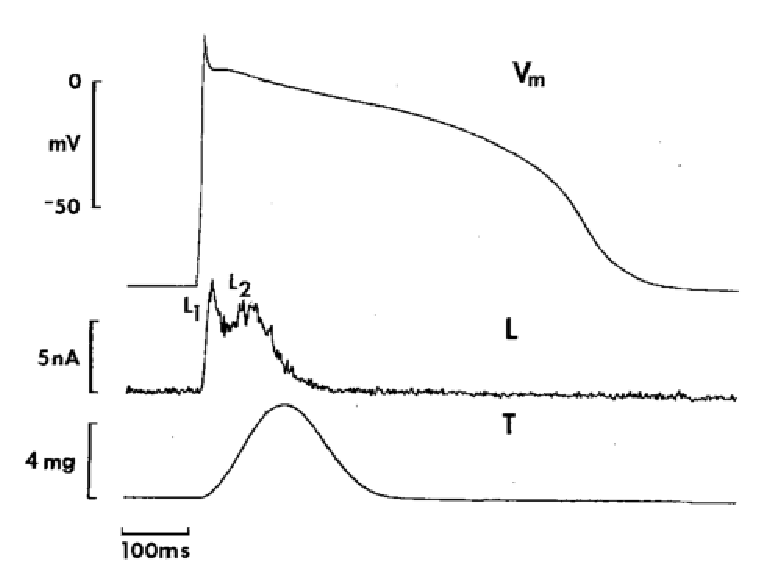
\includegraphics[height=3cm]{./images/Purkinjie_Calcium_Wier1982.eps}}
  \caption{The myosin is connected to the filament backbone by 2 springs. A
  thermal fluctuation has moved the myosin part toward the actin site, which is
  entering from the right. A further fluctuation can carry it to the position
  binding to actin traps. Then the relaxation of the springs drags the actin to
  the left.}
  \label{fig:motor_protein_Huxley}
\end{figure}

The mechanical coupling determines the velocity of length
changes. A muscle can shorten with a speed as a definite function of the
stimulus applied to it, e.g. Hill's relation (1938) was
\begin{equation}
P/P_o = \frac{1-V/V_\max}{1+(P_0/a)V/V_\max}
\end{equation}
with $P_0/a = 4$ (frog muscle at $0^\circ$C). Fenn-Marsh (1935) suggested
$P=W_0\exp(-aV)-kV$, with $W_0=0.95P_0, a=3.4/V_\max, k=0.03P_0/V_\max$
\citep{huxley1974}.

After a short delay of fluorescence elevation, the cell contract by about 8.6\%
in volume. Under AP, i.e. whole cell $\Ca$ elevation, the Fluo-3 fluorescence
start to rise after the electrical stimulus about 4ms, and reaches 90\% of peak
in 36ms, and the peak at 48ms \citep{cannell1994snu}. The cell contraction
starts later, i.e. at 34ms, reaching the value of 90\% maximum at 94ms and
peaking at 112ms, Fig.\ref{fig:global-transient_cannell1994}(B).
After the peak, the fluorescence decline with half-time decay $\tau = 138$ ms
and then contraction declines with half-time of 104ms. As shown in
Fig.\ref{fig:global-transient_cannell1994} (D), the uniformity increases with
time. At two different location (a) and (b), the time course of spark initiation
can be different, but after the peak, they are synchronzied and become very
similar.


\begin{figure}[hbt]
  \centerline{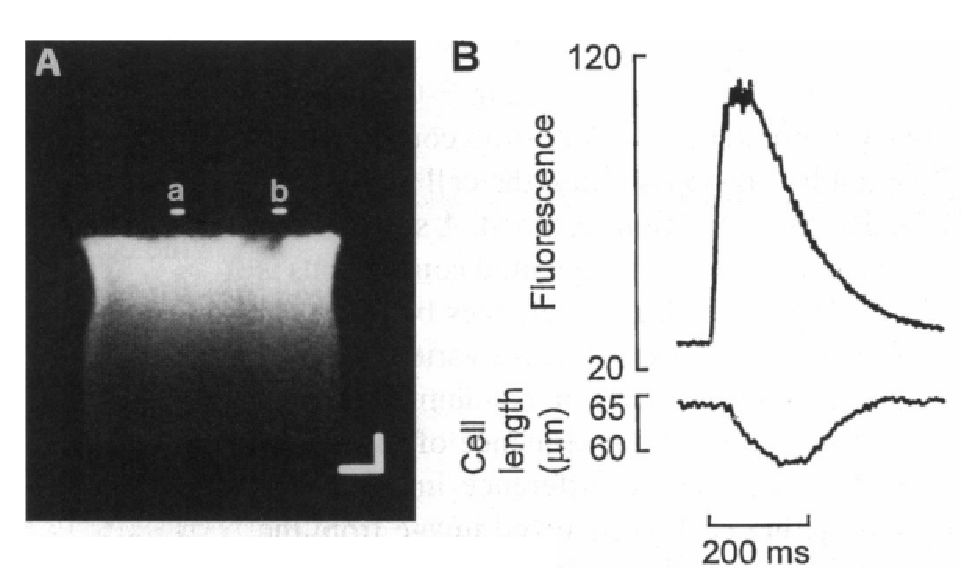
\includegraphics[height=5cm,
    angle=0]{./images/global_transient_cannell1994.eps}}
      \centerline{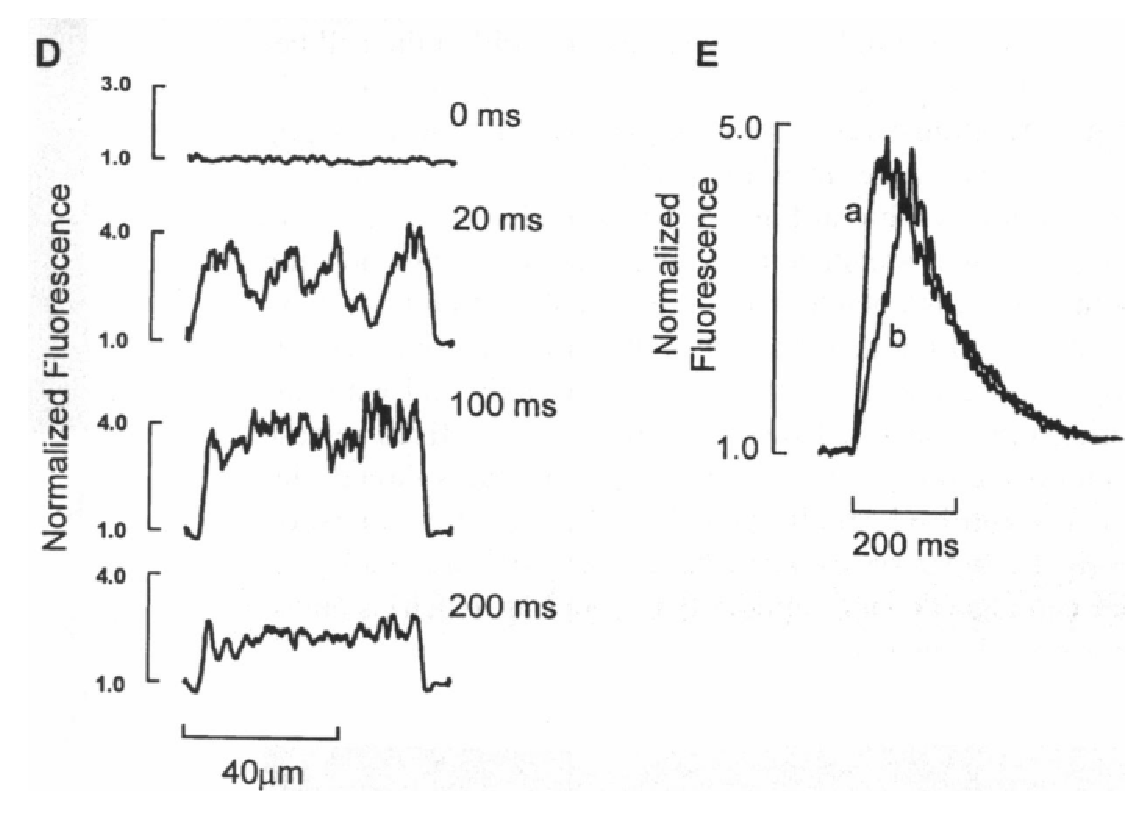
\includegraphics[height=3cm,
    angle=0]{./images/global_transient_normalized_cannell1994.eps}}
  \caption{(A) scale bar 20$\mum$ horizontal and 100ms vertical; (B) the time
  course of averaged fluorescence compared with contraction; (D) Normalized
  fluorescence F/F0 along the scan line at various time point after the
  stimulation, (E) the time course of average flurescence within the region
  indicated in (A) with 5.8$\mum$ wide}
  \label{fig:global-transient_cannell1994}
\end{figure}

\subsection{Mechanobiology and cardiac mechanotransduction}

{\bf Mechanobiology} is an emerging field at the interface of biology and
engineering. The major challenge is understanding {\it mechanotransduction} -
the molecular mechanism by which cells sense and respond to mechanical signals.
Even though this is a highly conserved process, the sensing mechanism can be
different in a single cell types, and among cell types. For a single cell type,
interestingly, the different forms of mechanotransduction is the result of
different signaling pathways. Also, the different forms of stretch can induce
different reactions. This requires studying individual cells independently.

{\bf Mechanosensation} (mes) is the transduction of mechanical force into a
cellular electrochemical signal. Apart from genetic change, it is suggested that
changes in cell mechanics, extracellular matrix structure, or
mechanotransduction can also contribute to the development of many diseases
(heart failure, cancer, asthma). We will focus on cardiac-related diseases.
Stretch was first reported to induce muscle growth in 1965 \citep{csapo1965}.
Then, there have been evidences of stretch-activated ion channels (SAC), calcium
spark rates, etc. Also, mechanical overload on cardiac myocytes after both
myocardial infarction and hypertension also induce hypertrophy. So, a mutation
in the gene responsible for mechanical stretch sensing can influence mechanical
stretch response and thus can lead to cardiac disease.

There are a vast number of mutations that are known to cause cardiac
disease, but the underlying mechanism from DNA mutation to the complex phenotype
is often unknown \citep{knoll2003}. The molecular identity of a mechanosensor in
cardiomyocytes is unknown. How the mechanotransduction occur can be modeled
using either two suggested approaches:
\begin{enumerate}
  \item localized (centralized) model: mechanotransduction trigger the cellular
  signal at the close proximity to the plasma membrane, i.e. stretch-activated
  channels (SAC). Potential proteins involving in mechanosensor are integrins,
  nonreceptor-type tyrosine kinases (Src).

  \item decentralized model: mechanotransduction is transmitted to other
  locations via the skeletons, and it then trigger signals at different
  subcellular regions. To describe the transmission of mechanical forces from
  one part of the cell to another, we use the term \verb!tensegrity!, i.e.
  tensegrity model of mechanotransduction.

  The important proteins involving in mechanotransduction at the sarcomere level
are, Fig.\ref{fig:sarcomere_protein}:
\begin{enumerate}
  \item Actin (thin filament)
  \item Myosin (thick filament)
  \item Proteins at the Z-disc:
  \begin{enumerate}
      \item $\alpha$-actinin
	  \item T-cap (19kDa): bind to Titin (thus giving it the name Titin-cap) and
	  other proteins ($\beta$-subunit minK potassium channel, MLP),
	  mutation in the gene cause a form of limb girdle muscular dystrophy
  	  \item MLP (26kDa muscle LIM protein): mice deficient for MLP cause a severe
  	  form of dilated cardiomyopathy (i.e. enlargement or impaired function of
  	  one or both ventricles). To rescue, an additional deletion with
  	  phospholamban can overcome the defect.
  	  \item Calsarcin-1
  \end{enumerate}
  \item Titin (giant protein spanning half sarcomere 4.2MDa) : is anchored at
  the Z-disc at the aminoterminal half, and bind to a variety of proteins
  ($\alpha$-actinine, T-cap).

  \item CARP (cardiac ankyrin repeat protein lies within I-band): may be involve
  in gene expression regulation.

  \item Melusin: bind to cytoplasmic domain of $\beta_1$ integrin. Deficiency of
  this protein haven't revealed any loss of function.

  \item Integrin: a group of transmembrane protein, possibly involving in
  mechanosensing
\end{enumerate}
The macromolecular complex (T-cap, MLP and Titin) functions as a stretch sensor.
\end{enumerate}
The two models can exist in parallel, and they may communicate.

\begin{figure}[hbt]
  \centerline{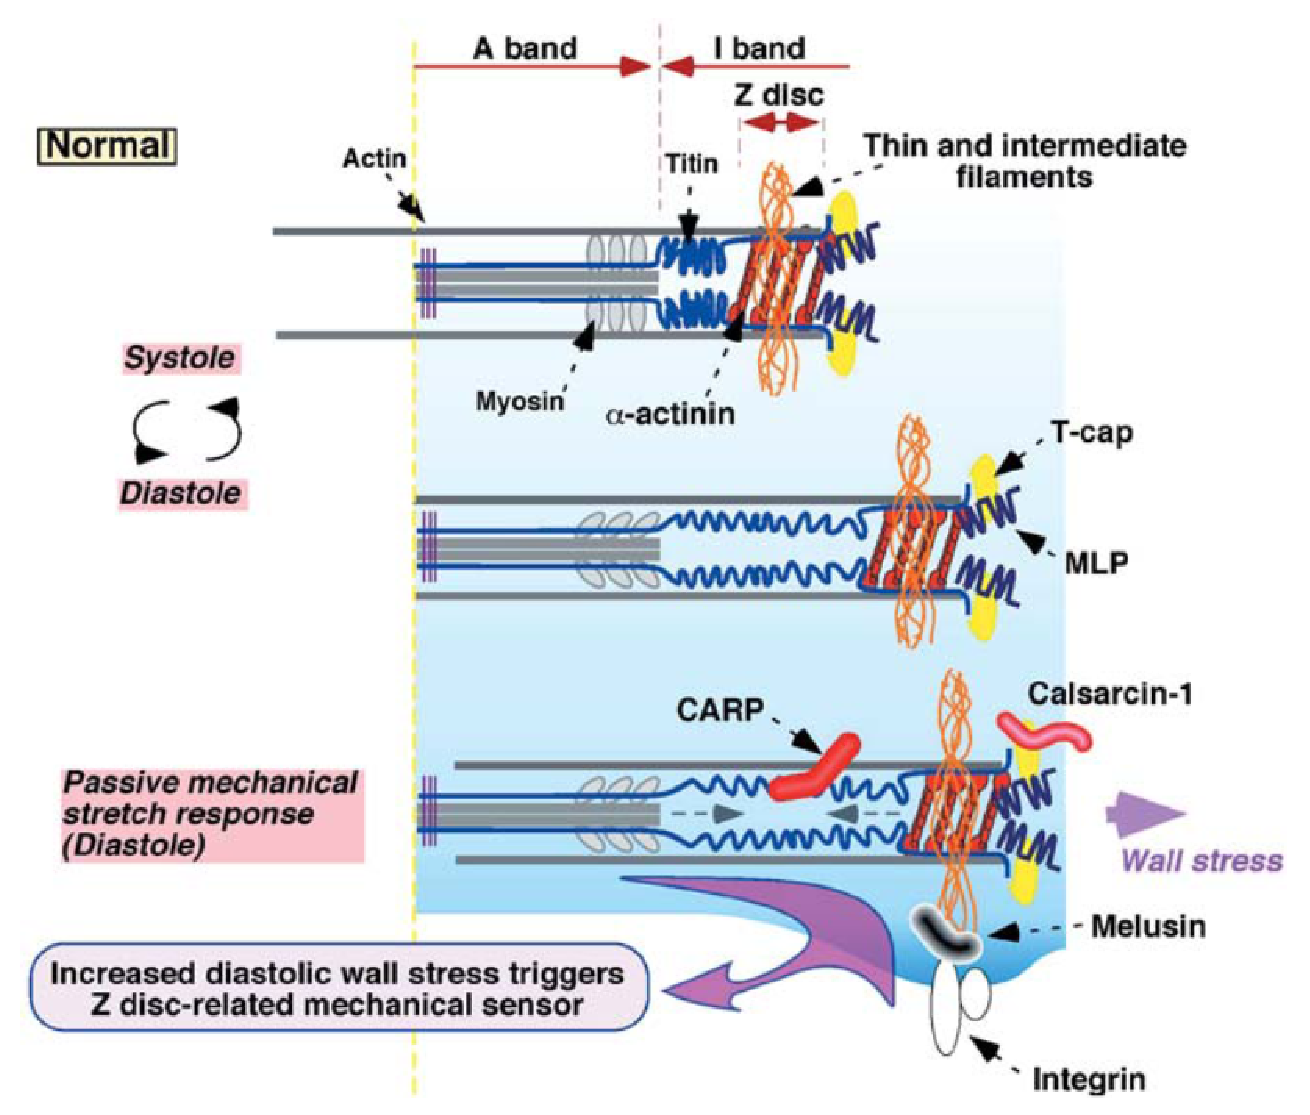
\includegraphics[height=5cm,
    angle=0]{./images/sarcomere_proteins.eps}}
  \caption{Schematic diagram of a half-sarcomere with different Z-disc proteins
  \citep{knoll2003}}
  \label{fig:sarcomere_protein}
\end{figure}

A small diastolic stretch (+8\%) induces an immediate, but short lasting (about
60s), increase in resting $\Ca$ sparks frequency (+30\%) \citep{iribe2009}.
Spark rate increase only in the stretched cell region, with non-significant
difference in spark amplitude, time to peak, and decay time constants of sparks
in stretched and non-stretched regions. It raised the question of mechanism for
immediate stretch response.
Iribe et a. suggested a linkage between cytoskeleton and RyR, when they found
tubulin filament right beside SR junctions and that microtubules physically
modulate RyR opening probability. These have been tested not the driver to the
increase in $\Ca$ sparks: stretch-activated channels (SAC), $\Ca$ influx, $\Na$
influx, NO signalling (nitric oxide) \citep{iribe2009}, acute stretch-induced
increase in SR calcium \citep{iribe2008}.

Recently, \citep{prosser2011} suggested that
a mechano-chemical signalling pathway that produce X-ROS (reactive oxygen
species) can be the transduction pathway for stretch-activated $\Ca$ sparks.
Early evidence showing two ROS-dependent processes: nitrosylation and oxidation
of RyR2 can contribute to aberrant SR $\Ca$ releases. {\it Duchene muscular
dystrophy} (DMD) is a stretch-sensitive muscular disorder.
The mouse model of DMD is {\it mdx} mouse.

\subsection{Starling law of the heart}

From experimental studies of isolated heart, Frank-Starling proposed a
hypothesis that the more blood coming in, the greater is the energy of the
contraction.
{\bf Starling law of the heart} (Frank-Starling law) stated that the strength of
the heart's systolic contraction is directly proportional to the diastolic
expansion; and under normal condition, the heart pumps out of the right atrium
all the blood given to it without letting any back-up in the veins.
So, in theory, the greater the amount of blood preload into the ventricle during
diastole, the greater the amount of blood ejected out of the heart during
systolic phase. This was widely appreciated by late 19th century physiologists.

The increase in volume stretches the ventricular wall. As such, a proper
stretching to the heart is very important to the normal supplying of blood to
the body. The heart is considered as a magic spring. The length-tension relation






\subsection{Rheology equation}

Rheology is the field that study the flow and deformation of matter, especially
fluid. Fluid is a substance that deforms continuously under the action of
shearing force. Complex fluids do not follow Newton's Law or Hooke's law (of
elasticity).



\section{Izakov et al. (1991)}

\citep{izakov1991} aimed to describe a number of known phenomenon in cardiac
muscle, including length-force and force-velocity relation. The essential
assumption is the isometric, isotonic and physiological condition of
contraction. The inactivation, i.e. the reduction of contractile capacity of
muscle depending on the mechanical conditions of contraction, is hypothesied
with two forms of cooperativity of proteins along the thin filaments in
sarcomeres.

The experiment data is from cat and rabbit pillary muscles.

\begin{figure}[hbt]
  \centerline{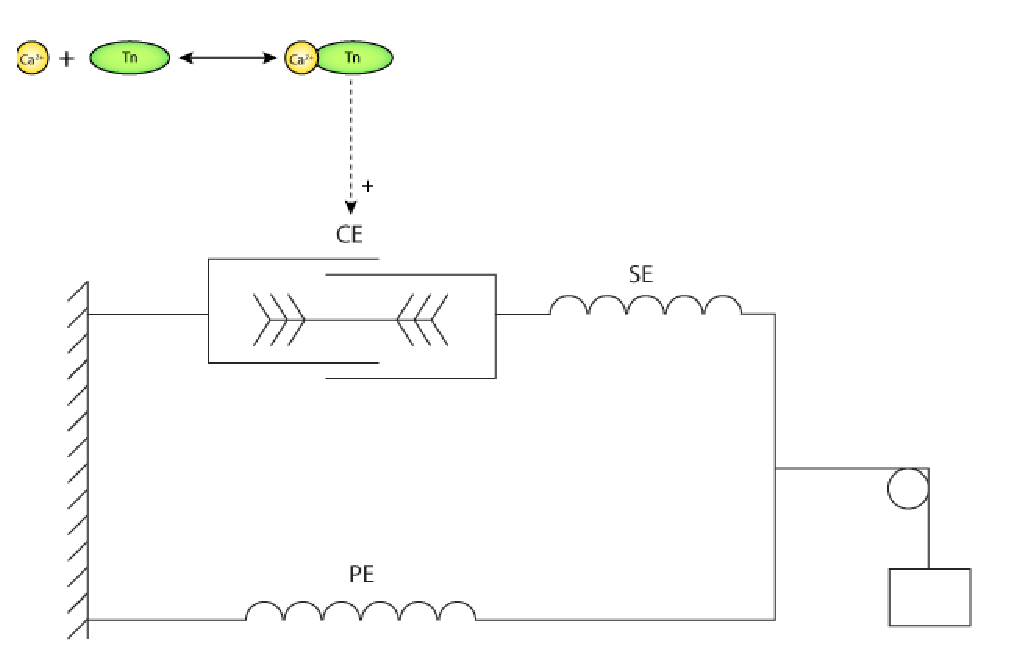
\includegraphics[height=5cm,
    angle=0]{./images/izakov_Force-Ca.eps}}
  \caption{}
  \label{fig:izakov_Force-Ca}
\end{figure}


Code:
\url{http://models.cellml.org/workspace/izakov_katsnelson_blyakhman_markhasin_shkylar_1991}


\section{Burkhoff (1994)}

\section{Landersberg-Sideman (1994)}



\section{Negroni-Lascano (1996)}

\citep{negroni1996} modeled the cross-bridge dynamics and intracellular $\Ca$
kinetics.

$\Ca$ kinetics is described by a 4-state system of sites on thin filament.


The model was able to reproduce:
\begin{enumerate}
  \item time course of isometric force: peak force 46.5 mN/mm$^2$
  \item intracellular $\Ca$: (peak is 1.5 $\muM$)
  \item force-length-$[\Ca]$ relation:
  \item transient response of force in response to step change in length
  \item force-velocity relation: maximum velocity 3 $\mum$/s
  \item force response to length pulse
  \item force response to quick release showing the superactivating and
  deactivating effects of shortening
  \item stiffness response to sinusoidal length change
  \item time course of active state
\end{enumerate}

\section{Hussan et al. (2006)}

\citep{hussan2006}
